% capitulo1.tex
\chapter{Nombre del capítulo}

\section{Xxxxxxxxx xxxxx xxxxxxxxxx}

Xxxxxxxxxxxxxxxxxxxxxxxxxxxxxxxxxxxxxxxxxxxxxxxxxxxxxxxxxxxxxxxxxxxxxxxxxxxxxxxxxxxxxxxxxxxxxxxxxxxxxxxxxxxxxxxxxxxxxxxxxxxxxxxxxxxxxxxxxxxxxxxxxxxxxxxxxxxxxxxxxxxxx.

Xxxxxxxxxxxxxxxxxxxxxxxxxxxxxxxxxxxxxxxxxxxxxxxxxxxxxxxxxxxxxxxxxxxxxxxxxxxxxxxxxxxxxxxxxxxxxxxxxxxxxxxxxxxxxxxxxxxxxxxxxxxxxxxxxxxxxxxxxxxxxxxxxxxxxxxxxxxxxxxxxxxxx.

\begin{table}[H]
\centering
\caption{Xxxxxxxx}
\label{tab:tabla1}
\begin{tabular}{@{}lcccc@{}}
\toprule
\multirow{2}{*}{\textbf{Internet}} & \multicolumn{2}{c}{\textbf{Urbano}} & \multicolumn{2}{c}{\textbf{Rural}} \\
\cmidrule(lr){2-3} \cmidrule(lr){4-5}
 & 06 a 09 & 10 a 11 & 06 a 09 & 10 a 11 \\
\midrule
Grado a & 10 & 15 & 2 & 4 \\
Grado b & 15 & 18 & 3 & 3 \\
Grado c & 15 & 10 & 3 & 1 \\
Grado d & 10 & 20 & 2 & 1 \\
\midrule
\textbf{Total} & 50 & 63 & 10 & 9 \\
\bottomrule
\end{tabular}
\vspace{0.5cm}\\
\textit{Nota}. Esta tabla se observa que los niños del sector urbano tienen mayor acceso al Internet.
\end{table}

\subsection{Xxxxxxxx xxxxxxxx xxxxxxxxxxx}

Xxxxxxxxxxxxxxxxxxxxxxxxxxxxxxxxxxxxxxxxxxxxxxxxxxxxxxxxxxxxxxxxxxxxxxxxxxxxxxxxxxxxxxxxxxxxxxx xxxxxxxxxxxxxx xxxxxxxx xxxxxxxxxxxxxxxxxxxxxxxxxxxxxxxxxxxx xxxxxxxxxxxx xxxxxxxxxxxxxxxxxxxxxx xxxxxxxxxxxxxxxxxxxxx.

\subsubsection{Xxxx xxxx xxxxxxx.} Xxxxxxxxxxxxxxxxxx xxxxx xxxxxx xxxxxxxxxxxxx xxxxxxxxxxxx.

\paragraph{Xxxx xxxxxxx xxx xxxx.} Xxxxxxxxxxxx xxxxxxxx xxxxxxxxxx xxxxxxx xxxxxxxxxxxx.

\begin{figure}[H]
\centering
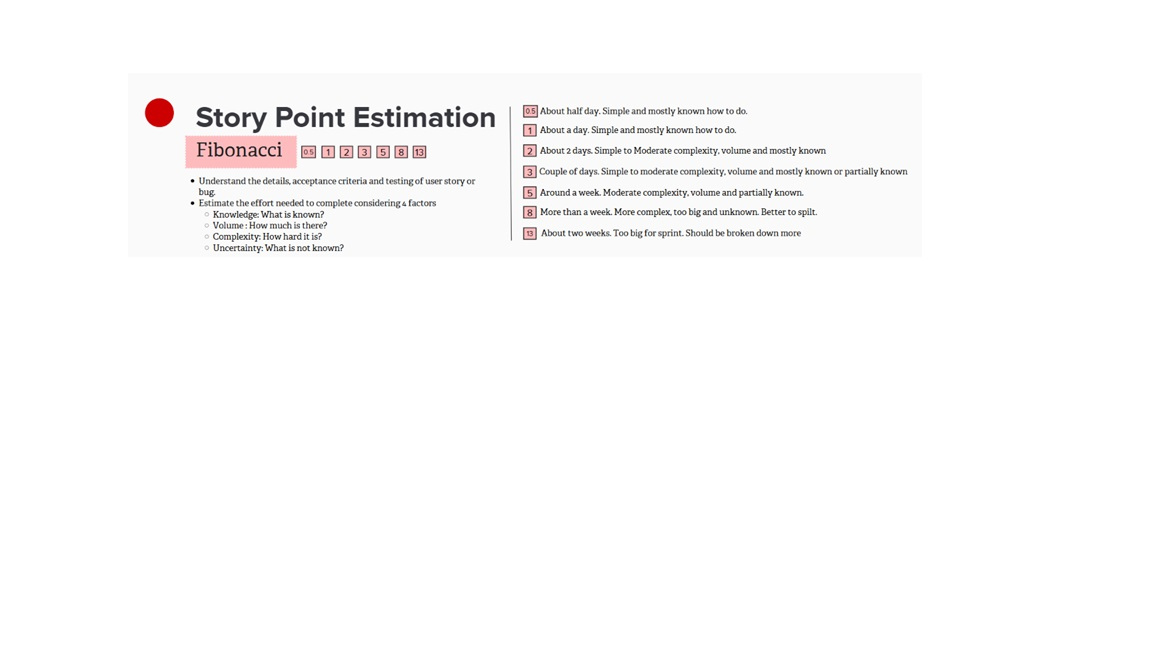
\includegraphics[width=0.7\textwidth]{figures/example.jpg}
\caption{Xxxxx}
\label{fig:figura1}
\textit{Nota}. Adaptado de Virus VIH [Fotografía], por Consejo Superior de Investigaciones Científicas, 2011, Flickr (flic.kr/p/aronSf). CC BY 2.0.
\end{figure}